\documentclass[a4paper,12pt]{article}
\usepackage[left=2cm,right=2cm,top=2cm,bottom=2cm]{geometry} % Do ustawień marginesów
\usepackage{multicol} % Dla podziału na kolumny
\usepackage{ragged2e} % Dla justowania tekstu
\usepackage{graphicx} % Required for inserting images
\usepackage{float}
\usepackage{caption}
\usepackage{amsmath} % Math formulas
\usepackage{amssymb} % Symbols
\usepackage[svgnames]{xcolor}
\usepackage[colorlinks=true, urlcolor=blue, linkcolor=black, citecolor=orange]{hyperref} % Hyperlinks
\usepackage{polski} % Polish language
\usepackage[utf8]{inputenc} % Text encoding
\usepackage{enumitem} % Pakiet do elastycznego sterowania listami
\usepackage{indentfirst}
\usepackage{array}
\usepackage{longtable}

\begin{document}

% Górna część strony
\noindent
\begin{minipage}{0.5\textwidth}
    \raggedright
    \textbf{Piotr Durniat} \\
    I rok, Fizyka \\
    Wtorek, 8:00-10:15 \\
    \vspace{0.5cm}
    \vspace{0.5cm}
\end{minipage}%
\begin{minipage}{0.5\textwidth}
    \raggedleft
    Data wykonania pomiarów: \\
    08.04.2025 \\
    \vspace{0.5cm} % Dodatkowa linia przerwy
    Prowadząca: \\
    dr Iwona Mróz
\end{minipage}

% Tytuł ćwiczenia
\vspace{2cm} % Odstęp
\begin{center}
    \LARGE \textbf{Ćwiczenie nr 19} \\[0.5cm]
    \Large \textbf{Pomiary stałej grawitacji G (ważenie Ziemi)}
\end{center}

% Reszta treści
\vspace{1cm} % Kolejny odstęp
\noindent

\tableofcontents
\newpage

% ---------- WSTĘP TEORETYCZNY ----------
\section{Wstęp teoretyczny}

\subsection*{Siła grawitacji}

Siłę grawitacji $F$ dla dwóch ciał o masach $m_1$ i $m_2$ oddalonych o $r$ można wyrazić wzorem:

\begin{equation}
    F = G \frac{m_1 m_2}{r^2}
\end{equation}

gdzie:
\begin{itemize}
    \item $G$ - stała grawitacji
\end{itemize}

\subsection*{Metoda wagi skręceń Cavendisha}

Metoda wagi skręceń Cavendisha jest jedną z metod wyznaczania stałej grawitacji $G$. Waga skręceń składa się z dwóch ciężarków o masie $m$ zawieszonych na obu końcach pręta, który jest zawieszony na cienkiej sprężystej nici będącej osią obrotu. W pobliżu tych kulek umieszcza się dwa duże ciężkie kulki o masie $M$. Wówczas siła grawitacji działająca na kulki $m$ wywołuje skręcenie nici aż do momentu, w którym siła grawitacji zrównoważy siłę sprężystości nici.

Mierząc okres drgań układu oraz odległość między wychyleniami masy $m$ względem położenia równowagi w dwóch różnych ustawieniach masy $M$ można wyznaczyć stałą grawitacji $G$ ze wzoru:

\begin{equation}
    \label{eq:g_cavendish}
    G = \frac{\pi^2 r^2 d \Delta b}{MT^2 L}
\end{equation}

gdzie:
\begin{itemize}
    \setlength{\itemsep}{0em}
    \item $L = 0,86\text{ m}$ - odległość zwierciadła od ekranu 
    \item $r = 0,045\text{ m}$ - odległość między środkami mas $M$ i $m$
    \item $d = 0,05\text{ m}$ - odległość małej kulki od osi obrotu
    \item $M = 1,5\text{ kg}$ - masa dużej kulki
    \item $T$ - okres drgań układu (wyznaczony w doświadczeniu)
    \item $\Delta b$ - Różnica między wychyleniami masy $m$ względem położenia równowagi w dwóch różnych ustawieniach masy $M$ (wyznaczona w doświadczeniu)
\end{itemize}


Wstęp teoretyczny opracowano na podstawie materiałów pomocniczych do ćwiczenia~\cite{materialy_pomoc_19}.


% ---------- OPIS DOŚWIADCZENIA ----------
\section{Opis doświadczenia}

\begin{enumerate}
    \item Obserwacja początkowego położenia plamki świetlnej na skali.
    \item Ustawienie dużych kul w pierwszym skrajnym położeniu (wykonywane przez prowadzącego).
    \item Rejestrowanie położenia plamki na skali co 30 sekund przez około 30 minut.
    \item Przesunięcie dużych kul do drugiego skrajnego położenia (wykonywane przez prowadzącego).
    \item Powtórne rejestrowanie położenia plamki co 30 sekund przez około 30 minut.
    \item Sporządzenie wykresów ruchu wahadła dla obu ustawień kul.
    \item Wyznaczenie maksimów i minimów oscylacji wahadła.
    \item Obliczenie położenia środków wahań dla obu ustawień kul.
    \item Wyznaczenie różnicy położeń środków wahań $\Delta b$.
    \item Obliczenie stałej grawitacji $G$ na podstawie uzyskanych pomiarów.
    \item Oszacowanie masy Ziemi przy użyciu wyznaczonej wartości $G$.
\end{enumerate}

% ---------- OPRACOWANIE WYNIKÓW POMIARÓW ----------
\section{Opracowanie wyników pomiarów}

% ---------- TABELE ----------
\subsection{Tabele pomiarowe}
\renewcommand{\arraystretch}{0.85}

\begin{longtable}{|c|c|c|c|}
\hline
\textbf{lp} & \textbf{Czas [t] w min} & \textbf{Położenie plamki 1} & \textbf{Położenie plamki 2} \\
\hline
\endfirsthead
\hline
\textbf{lp} & \textbf{Czas [t] w min} & \textbf{Położenie plamki 1} & \textbf{Położenie plamki 2} \\
\hline
\endhead
1 & 00:00:00 & 10 & 30 \\ \hline
2 & 00:00:30 & 5  & 35 \\ \hline
3 & 00:01:00 & 5  & 45 \\ \hline
4 & 00:01:30 & 5  & 55 \\ \hline
5 & 00:02:00 & 5  & 60 \\ \hline
6 & 00:02:30 & 10 & 70 \\ \hline
7 & 00:03:00 & 15 & 80 \\ \hline
8 & 00:03:30 & 20 & 75 \\ \hline
9 & 00:04:00 & 25 & 60 \\ \hline
10 & 00:04:30 & 30 & 50 \\ \hline
11 & 00:05:00 & 40 & 35 \\ \hline
12 & 00:05:30 & 40 & 30 \\ \hline
13 & 00:06:00 & 45 & 25 \\ \hline
14 & 00:06:30 & 45 & 25 \\ \hline
15 & 00:07:00 & 45 & 30 \\ \hline
16 & 00:07:30 & 40 & 40 \\ \hline
17 & 00:08:00 & 40 & 45 \\ \hline
18 & 00:08:30 & 35 & 55 \\ \hline
19 & 00:09:00 & 30 & 70 \\ \hline
20 & 00:09:30 & 25 & 80 \\ \hline
21 & 00:10:00 & 20 & 80 \\ \hline
22 & 00:10:30 & 20 & 75 \\ \hline
23 & 00:11:00 & 15 & 70 \\ \hline
24 & 00:11:30 & 15 & 65 \\ \hline
25 & 00:12:00 & 15 & 60 \\ \hline
26 & 00:12:30 & 20 & 55 \\ \hline
27 & 00:13:00 & 20 & 55 \\ \hline
28 & 00:13:30 & 20 & 50 \\ \hline
29 & 00:14:00 & 25 & 50 \\ \hline
30 & 00:14:30 & 30 & 50 \\ \hline
31 & 00:15:00 & 30 & 55 \\ \hline
32 & 00:15:30 & 35 & 55 \\ \hline
33 & 00:16:00 & 35 & 60 \\ \hline
34 & 00:16:30 & 35 & 65 \\ \hline
35 & 00:17:00 & 40 & 70 \\ \hline
36 & 00:17:30 & 35 & 70 \\ \hline
37 & 00:18:00 & 35 & 75 \\ \hline
38 & 00:18:30 & 35 & 75 \\ \hline
39 & 00:19:00 & 30 & 75 \\ \hline
40 & 00:19:30 & 30 & 75 \\ \hline
41 & 00:20:00 & 25 & 75 \\ \hline
42 & 00:20:30 & 20 & 70 \\ \hline
43 & 00:21:00 & 20 & 70 \\ \hline
44 & 00:21:30 & 20 & 65 \\ \hline
45 & 00:22:00 & 20 & 65 \\ \hline
46 & 00:22:30 & 20 & 60 \\ \hline
47 & 00:23:00 & 20 & 60 \\ \hline
48 & 00:23:30 & 20 & 60 \\ \hline
49 & 00:24:00 & 25 & 55 \\ \hline
50 & 00:24:30 & 25 & 55 \\ \hline
51 & 00:25:00 & 25 & 55 \\ \hline
52 & 00:25:30 & 30 & 60 \\ \hline
53 & 00:26:00 & 30 & 60 \\ \hline
54 & 00:26:30 & 30 & 65 \\ \hline
55 & 00:27:00 & 30 & 65 \\ \hline
56 & 00:27:30 & 35 & 65 \\ \hline
57 & 00:28:00 & 30 & 70 \\ \hline
58 & 00:28:30 & 30 & 70 \\ \hline
59 & 00:29:00 & 30 & 70 \\ \hline
60 & 00:29:30 & 30 & 70 \\ \hline
61 & 00:30:00 & 25 & 70 \\ \hline
\end{longtable}

\renewcommand{\arraystretch}{1}

% ---------- OBLICZENIA ----------
\subsection{Wyznaczanie położeń środkowych}

Wykreślono pomiary na wykresie \ref{fig:wykres} i wyznaczono ekstrema. Następnie wyznaczono położenia środków wahań dla obu ustawień kul na podstawie wzoru:
\begin{align*}
    b_{01} & = \frac{\frac{b_1+b_3}{2}+b_2}{2} = \frac{b_1}{4} + \frac{b_2}{2} + \frac{b_3}{4} \rightarrow \text{pierwsze ustawienie}; \\
    b_{02} & = \frac{\frac{b_1+b_3}{2}+b_2}{2} = \frac{b_1}{4} + \frac{b_2}{2} + \frac{b_3}{4} \rightarrow \text{drugie ustawienie}.
\end{align*}

gdzie $b_1, b_2, b_3$ to odpowiednio maximum, następujące po nim minimum i następne maximum dla danego ustawienia.
Wybrane ekstrema to:

\begin{itemize}
    \item Pierwsze ustawienie: $b_1 = 45$ mm, $b_2 = 15$ mm, $b_3 = 40$ mm
    \item Drugie ustawienie: $b_1 = 80$ mm, $b_2 = 50$ mm, $b_3 = 75$ mm
\end{itemize}

Po podstawieniu do wzorów na położenia środkowe otrzymujemy:
\begin{align*}
    b_{01} &= \frac{45}{4} + \frac{15}{2} + \frac{40}{4} = 28{,}75 \text{ mm} \\
    b_{02} &= \frac{80}{4} + \frac{50}{2} + \frac{75}{4} = 63{,}75 \text{ mm}
\end{align*}

Różnica między położeniami środkowymi wynosi:
\begin{equation*}
    \Delta b = b_{02} - b_{01} = 63{,}75 - 28{,}75 = 35 \text{ mm}
\end{equation*}


\subsection{Wyznaczanie okresu drgań}

Okres drgań został wyznaczony jako odległość czasu pomiędzy wybranymi maksimami i minimami oscylacji wahadła. Wybrano 4 pary następujących po sobie ekstremów w obu ustawieniach i okres drań dla nich wszystkich wyniósł:

\begin{align*}
T_1 & = 17,0 - 6,5 = 10,5 \text{ s} \\
T_2 & = 27,5 - 17,0 = 10,5 \text{ s} \\
T_3 & = 11,5 - 1,0 = 10,5 \text{ s} \\
T_4 & = 24,5 - 14,0 = 10,5 \text{ s}
\end{align*}

Jak widać dla wszystkich przypadków okres drgań wyniósł $10,5$ sekundy.

\subsection{Wyznaczanie stałej grawitacji}

Niepewność pomiaru stałej grawitacji wyznaczamy korzystając ze wzoru (18) z instrukcji ONP:

\begin{equation}
\Delta y = \sum_{k=1}^{K} \left| \frac{\partial f}{\partial x_k} \Delta x_k \right|
\end{equation}

Podstawiając wzór na stałą grawitacji:

\begin{equation}
G = \frac{\pi^2 r^2 d \Delta b}{MT^2L}
\end{equation}

Wyznaczamy odpowiednie pochodne cząstkowe:

\begin{align}
\frac{\partial G}{\partial \Delta b} &= \frac{\pi^2 r^2 d}{MT^2L} = \frac{G}{\Delta b} \\[8pt]
\frac{\partial G}{\partial T} &= \frac{-2\pi^2 r^2 d \Delta b}{MT^3L} = \frac{-2G}{T}
\end{align}

Uwzględniając największy wpływ niepewności wyznaczenia $\Delta b$ oraz okresu drgań $T$, otrzymujemy:

\begin{equation}
\Delta G = \left| \frac{\partial G}{\partial T} \Delta T \right| + \left| \frac{\partial G}{\partial \Delta b} \Delta(\Delta b) \right| = \left| \frac{-2G}{T} \Delta T \right| + \left| \frac{G}{\Delta b} \Delta(\Delta b) \right|
\end{equation}

Podstawiając wartości liczbowe:

\begin{align}
\Delta G &= \left| \frac{-2 \cdot 7{,}45 \cdot 10^{-11}}{630} \cdot 60 \right| + \left| \frac{7{,}45 \cdot 10^{-11}}{0{,}035} \cdot 0{,}010 \right| \\[8pt]
&= 1{,}42 \cdot 10^{-12} + 2{,}13 \cdot 10^{-11} \\[8pt]
&= 2{,}27 \cdot 10^{-11} \frac{\text{m}^3}{\text{kg} \cdot \text{s}^2}
\end{align}

Zatem niepewność wyznaczenia stałej grawitacji wynosi:

\begin{equation}
\Delta G = 2{,}27 \cdot 10^{-11} \frac{\text{m}^3}{\text{kg} \cdot \text{s}^2}
\end{equation}

\subsection{Wyznaczanie masy Ziemi}


Siła grawitacji $F$ działająca na masę $m$ na powierzchni Ziemi wynosi:
\begin{equation}
    \label{eq:f_ziemia}
F = G \frac{mM_Z}{R_Z^2}
\end{equation}
gdzie $M_Z$ to masa Ziemi, $R_Z$ to promień Ziemi.

Siła z jaką Ziemia przyciąga masę $m$ wynosi:
\begin{equation}
    \label{eq:f_ziemia_2}
F = mg
\end{equation}

Stąd porównując wzory \eqref{eq:f_ziemia} i \eqref{eq:f_ziemia_2} otrzymujemy:

\begin{align*}
    & mg = G \frac{mM_Z}{R_Z^2} \Rightarrow \\
    & M_Z = \frac{gR_Z^2}{G}
\end{align*}

Podstawiając wartości liczbowe:

\begin{align*}
    M_Z &= \frac{9{,}81 \cdot (6{,}38 \cdot 10^6)^2}{7{,}45 \cdot 10^{-11}} \\
    &= 5{,}36 \cdot 10^{24} \text{ kg}
\end{align*}










% ---------- NIEPEWNOŚCI ----------
\section{Ocena niepewności pomiaru}

\subsection{Niepewność $\Delta b$}

Niepewność wzorcowania dla każdego z pomiarów $b_1, b_2, b_3$ wynosi:

$$
\Delta b_x = 0,005 \text{ mm}
$$

Niepewność położenia środka wahań (dla obu ustawień) została obliczona na podstawie wzoru:

$$
b_{0x} = \frac{b_1}{4} + \frac{b_2}{2} + \frac{b_3}{4}
$$

stąd maksymalna niepewność $\Delta b_{0x}$ wynosi:

$$
\Delta b_{0x} = \frac{1}{4}\Delta b_x + \frac{1}{2}\Delta b_x + \frac{1}{4}\Delta b_x = \Delta b_x
$$

$\Delta b$ zostało obliczone na podstawie wzoru:

$$
\Delta b = b_{02} - b_{01}
$$

stąd maksymalna niepewność $\Delta(\Delta b)$ wynosi:
\begin{align*}
\Delta(\Delta b) &= |1 \cdot \Delta b_{02}| + |(-1) \cdot \Delta b_{01}| = \Delta b_{02} + \Delta b_{01} = 2\Delta b_x \\
&= 0,010 \text{ mm}
\end{align*}


\subsection{Niepewność $T$}

Pomiary były wykonywane co 30 sekund, więc niepewność pomiaru czasu wynosi $\Delta t = 30 \text{ s}$.
Okres został obliczony jako różnica między dwoma pomiarami czasu, stąd jej niepewność wynosi:

$$
\Delta T = 2 \cdot 30 \text{ s} = 60 \text{ s}
$$

\subsection{Niepewność $G$}

Niepewność pomiaru stałej grawitacji wyznaczamy korzystając ze wzoru (18) z instrukcji ONP:

\begin{equation*}
\label{eq:delta_y}
\Delta y = \sum_{k=1}^{K} \left| \frac{\partial f}{\partial x_k} \Delta x_k \right|
\end{equation*}

Podstawiając wzór na stałą grawitacji:

\begin{equation*}
\label{eq:g}
G = \frac{\pi^2 r^2 d \Delta b}{MT^2L}
\end{equation*}

Wyznaczamy odpowiednie pochodne cząstkowe:

\begin{equation*}
\frac{\partial G}{\partial \Delta b} = \frac{\pi^2 r^2 d}{MT^2L} = \frac{G}{\Delta b}
\end{equation*}

\begin{equation*}
\frac{\partial G}{\partial \Delta T} = \frac{-2\pi^2 r^2 d}{MT^3L} = \frac{-2G}{T}
\end{equation*}

Uwzględniając największy wpływ niepewności wyznaczenia $\Delta b$ oraz okresu drgań $T$, otrzymujemy:

\begin{equation*}
\Delta G = | \frac{-2G}{T} \Delta T | + | \frac{G}{\Delta b} \Delta( \Delta b ) |
\end{equation*}

Podstawiając wartości liczbowe:

\begin{equation*}
\Delta G = | \frac{-2 \cdot 7{,}45 \cdot 10^{-11}}{630} \cdot 60 | + | \frac{7{,}45 \cdot 10^{-11}}{0{,}035} \cdot 0{,}010 |
= 3{,}55 \cdot 10^{-11} \frac{\text{m}^3}{\text{kg} \cdot \text{s}^2}
\end{equation*}



% ---------- WNIOSKI ----------
\section{Wnioski}

\begin{enumerate}
    \item Obliczona wartość stałej grawitacji wynosi $7{,}45 \cdot 10^{-11} \frac{\text{m}^3}{\text{kg} \cdot \text{s}^2}$ z niepewnością maksymalną $3{,}55 \cdot 10^{-11} \frac{\text{m}^3}{\text{kg} \cdot \text{s}^2}$. Rzeczywista wartość stałej grawitacji wynosi $6{,}67 \cdot 10^{-11} \frac{\text{m}^3}{\text{kg} \cdot \text{s}^2}$, co mieści się w przedziale niepewności.

    \item Obliczona wartość masy Ziemi wynosi $5{,}36 \cdot 10^{24} \text{ kg}$. Rzeczywista wartość masy Ziemi wynosi $5{,}98 \cdot 10^{24} \text{ kg}$.

    \item Główne źródła niepewności w pomiarze to:
    \begin{itemize}
        \item Duża niepewność pomiaru czasu ($\Delta T = 60$ s), która wynikała z przyjętego interwału pomiarowego (co 30 s).
        \item Wpływ czynników zewnętrznych (drgania podłoża, ruchy powietrza), które mogły zaburzać ruch wahadła pomimo osłony szklanej.
        \item Trudności w precyzyjnym odczytaniu położenia plamki na skali (przyjęto niepewność $0{,}050$ mm).
    \end{itemize}

    \item Otrzymane wyniki potwierdzają słuszność prawa powszechnego ciążenia Newtona.
\end{enumerate}
\newpage

% ---------- WYKRESY ----------
\section{Wykresy}

\begin{figure}[H]
    \centering
    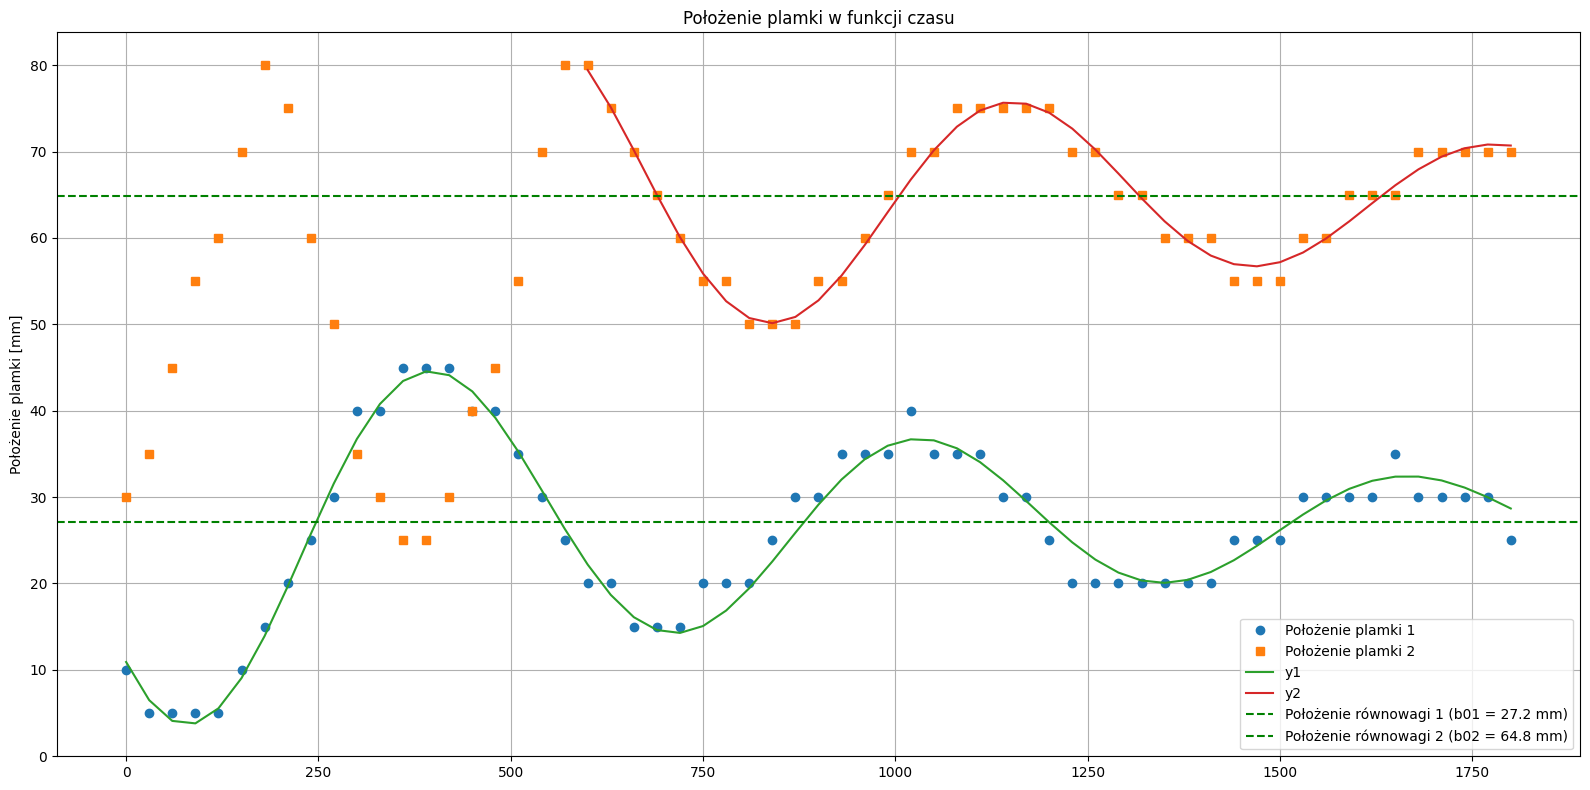
\includegraphics[width=0.9\textheight,angle=90]{wykres.png}
    \caption{Wykres zależności wychylenia od czasu (źródło: opracowanie własne)}
    \label{fig:wykres}
\end{figure}


\bibliographystyle{plain}
\bibliography{bibliography}

\end{document}
